
\documentclass[border=10pt]{standalone}
\usepackage{amsmath}
\usepackage{tikz}
\usetikzlibrary{patterns, calc}

\begin{document}
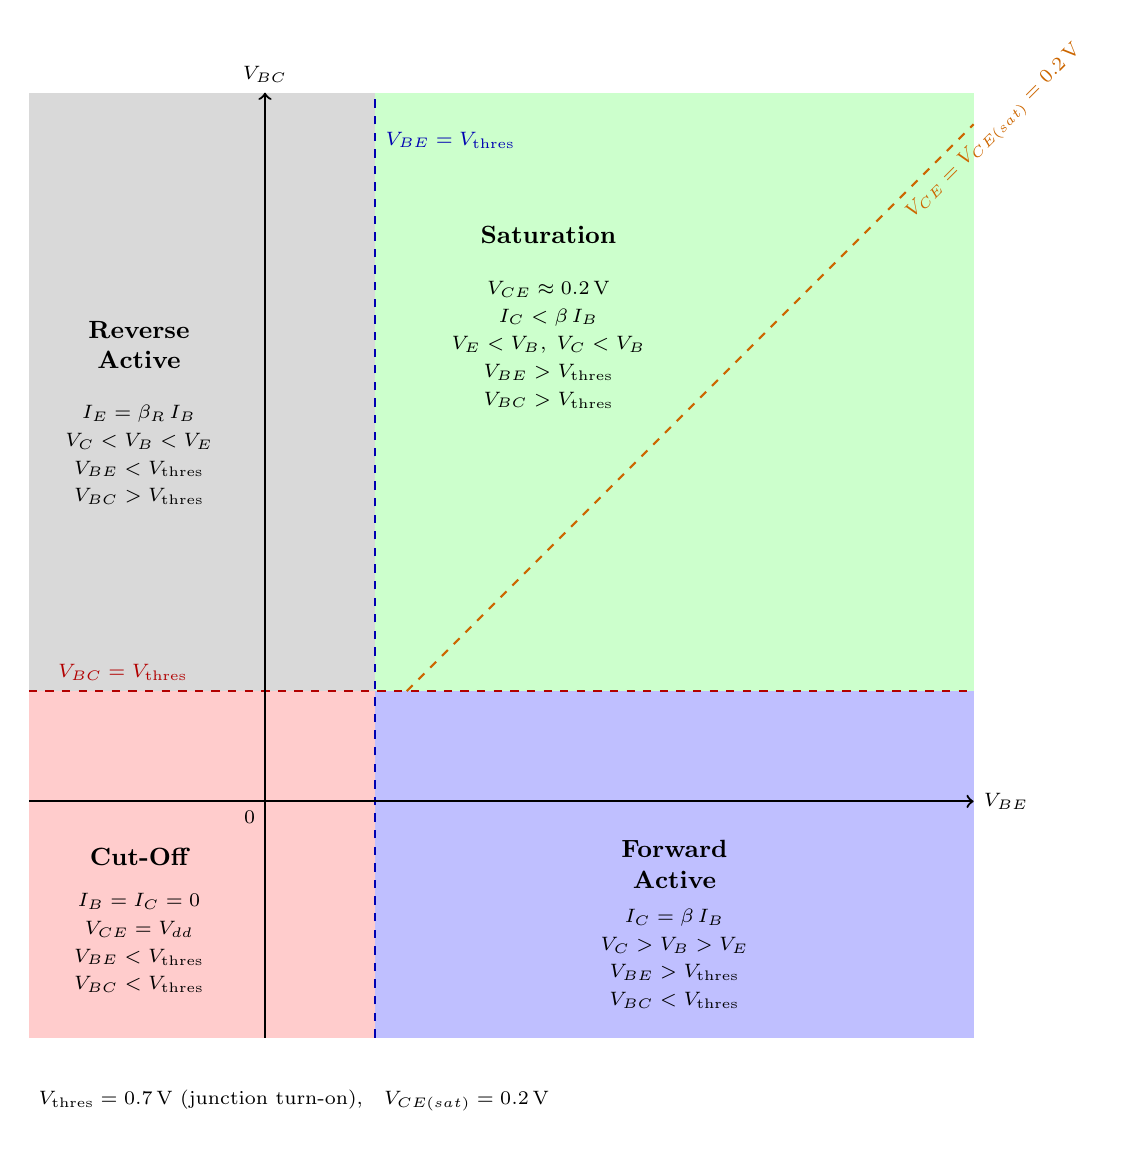
\begin{tikzpicture}[scale=2.0, every node/.style={font=\scriptsize}]

    % === Axis limits ===
    \def\xmin{-1.5}  \def\xmax{4.5}
    \def\ymin{-1.5}  \def\ymax{4.5}
    \def\Von{0.7}    % junction turn-on voltage
    \def\Vcesat{0.2} % VCE(sat)

    % === Region fills ===
    % Cut-off (bottom-left)
    \fill[red!20] (\xmin,\ymin) rectangle (\Von,\Von);
    % Forward Active (bottom-right)
    \fill[blue!25] (\Von,\ymin) rectangle (\xmax,\Von);
    % Reverse Active (top-left)
    \fill[gray!30] (\xmin,\Von) rectangle (\Von,\ymax);
    % Saturation (top-right)
    \fill[green!20] (\Von,\Von) rectangle (\xmax,\ymax);

    % === VCE = 0.2V diagonal (VBC = VBE - 0.2) ===
    % This line further divides the saturation/active boundary
    \draw[thick, dashed, orange!80!black]
    (\Von + \Vcesat, \Von) -- (\xmax, \xmax - \Vcesat)
    node[pos=0.85, below right, rotate=45, font=\scriptsize]
    {$V_{CE} = V_{CE(sat)} = 0.2\,\text{V}$};

    % === Threshold lines ===
    \draw[thick, dashed, blue!70!black]
    (\Von, \ymin) -- (\Von, \ymax)
    node[pos=0.95, right, font=\scriptsize] {$V_{BE} = V_{\text{thres}}$};
    \draw[thick, dashed, red!70!black]
    (\xmin, \Von) -- (\xmax, \Von)
    node[pos=0.02, above right, font=\scriptsize] {$V_{BC} = V_{\text{thres}}$};

    % === Axes ===
    \draw[->, thick] (\xmin,0) -- (\xmax,0) node[right] {$V_{BE}$};
    \draw[->, thick] (0,\ymin) -- (0,\ymax) node[above] {$V_{BC}$};

    % === Region labels ===
    % Cut-off
    \node[align=center, font=\small\bfseries] at ({(\xmin+\Von)/2 - 0.4}, {(\ymin+\Von)/2 +0.05})
    {Cut-Off};
    \node[align=center, font=\scriptsize] at ({(\xmin+\Von)/2 - 0.4}, {(\ymin+\Von)/2 - 0.5})
    {$I_B = I_C = 0$\\[2pt]$V_{CE} = V_{dd}$\\[2pt]$V_{BE} < V_{\text{thres}}$\\[2pt]$V_{BC} < V_{\text{thres}}$};

    % Forward Active
    \node[align=center, font=\small\bfseries] at ({(\Von+\xmax)/2}, {(\ymin+\Von)/2})
    {Forward\\Active};
    \node[align=center, font=\scriptsize] at ({(\Von+\xmax)/2}, {(\ymin+\Von)/2 - 0.6})
    {$I_C = \beta\, I_B$\\[2pt]$V_C > V_B > V_E$\\[2pt]$V_{BE} > V_{\text{thres}}$\\[2pt]$V_{BC} < V_{\text{thres}}$};

    % Saturation (shifted to top-left of quadrant, away from diagonal)
    \node[align=center, font=\small\bfseries] at (1.8, 3.6)
    {Saturation};
    \node[align=center, font=\scriptsize] at (1.8, 2.9)
    {$V_{CE} \approx 0.2\,\text{V}$\\[2pt]$I_C < \beta\, I_B$\\[2pt]$V_E < V_B,\; V_C < V_B$\\[2pt]$V_{BE} > V_{\text{thres}}$\\[2pt]$V_{BC} > V_{\text{thres}}$};

    % Reverse Active
    \node[align=center, font=\small\bfseries] at ({(\xmin+\Von)/2 - 0.4}, {(\Von+\ymax)/2 + 0.3})
    {Reverse\\Active};
    \node[align=center, font=\scriptsize] at ({(\xmin+\Von)/2 - 0.4}, {(\Von+\ymax)/2 - 0.4})
    {$I_E = \beta_R\, I_B$\\[2pt]$V_C < V_B < V_E$\\[2pt]$V_{BE} < V_{\text{thres}}$\\[2pt]$V_{BC} > V_{\text{thres}}$};

    % === Origin label ===
    \node[below left, font=\scriptsize] at (0,0) {$0$};

    % === Legend ===
    \node[font=\scriptsize, anchor=west] at (\xmin, \ymin - 0.4)
    {$V_{\text{thres}} = 0.7\,\text{V}$ (junction turn-on), \;
        $V_{CE(sat)} = 0.2\,\text{V}$};

\end{tikzpicture}
\end{document}